\section{CUDA运行时API详解与设备属性查询}

大家好，在今天的文章中我将解释CUDA运行时API（RuntimeAPI）。CUDA运行时API为CUDA提供了一个高级
接口，它使开发者能够高效地利用NVIDIA GPU的能力来完成广泛的计算任务。这些API简化了管理GPU设备、内存分配以及
执行并行内核的过程。

运行时API可供程序员用来开发优化或运行GPU加速的应用程序。这种方法是一个省时的替代方案，无需阅读GPU白皮书中详细的
文档。例如，无需深入研究白皮书来查找设备限制和约束。就像我们在前一节中解释的那样，例如每个块的最大线程数，这些API提供
了函数，允许你直接从GPU查询那个值。

让我们来查看这个专门用于运行时API函数的网页。如这个网页所示，我们有数十个函数，涵盖设备管理（例如这个函数）、内存处理
（比如这一个）以及异步计算。如果你想从运行时API中找到任何函数，你需要来到这个网页。

\subsection{核心函数：cudaGetDeviceProperties}

\begin{figure}
    \centering
    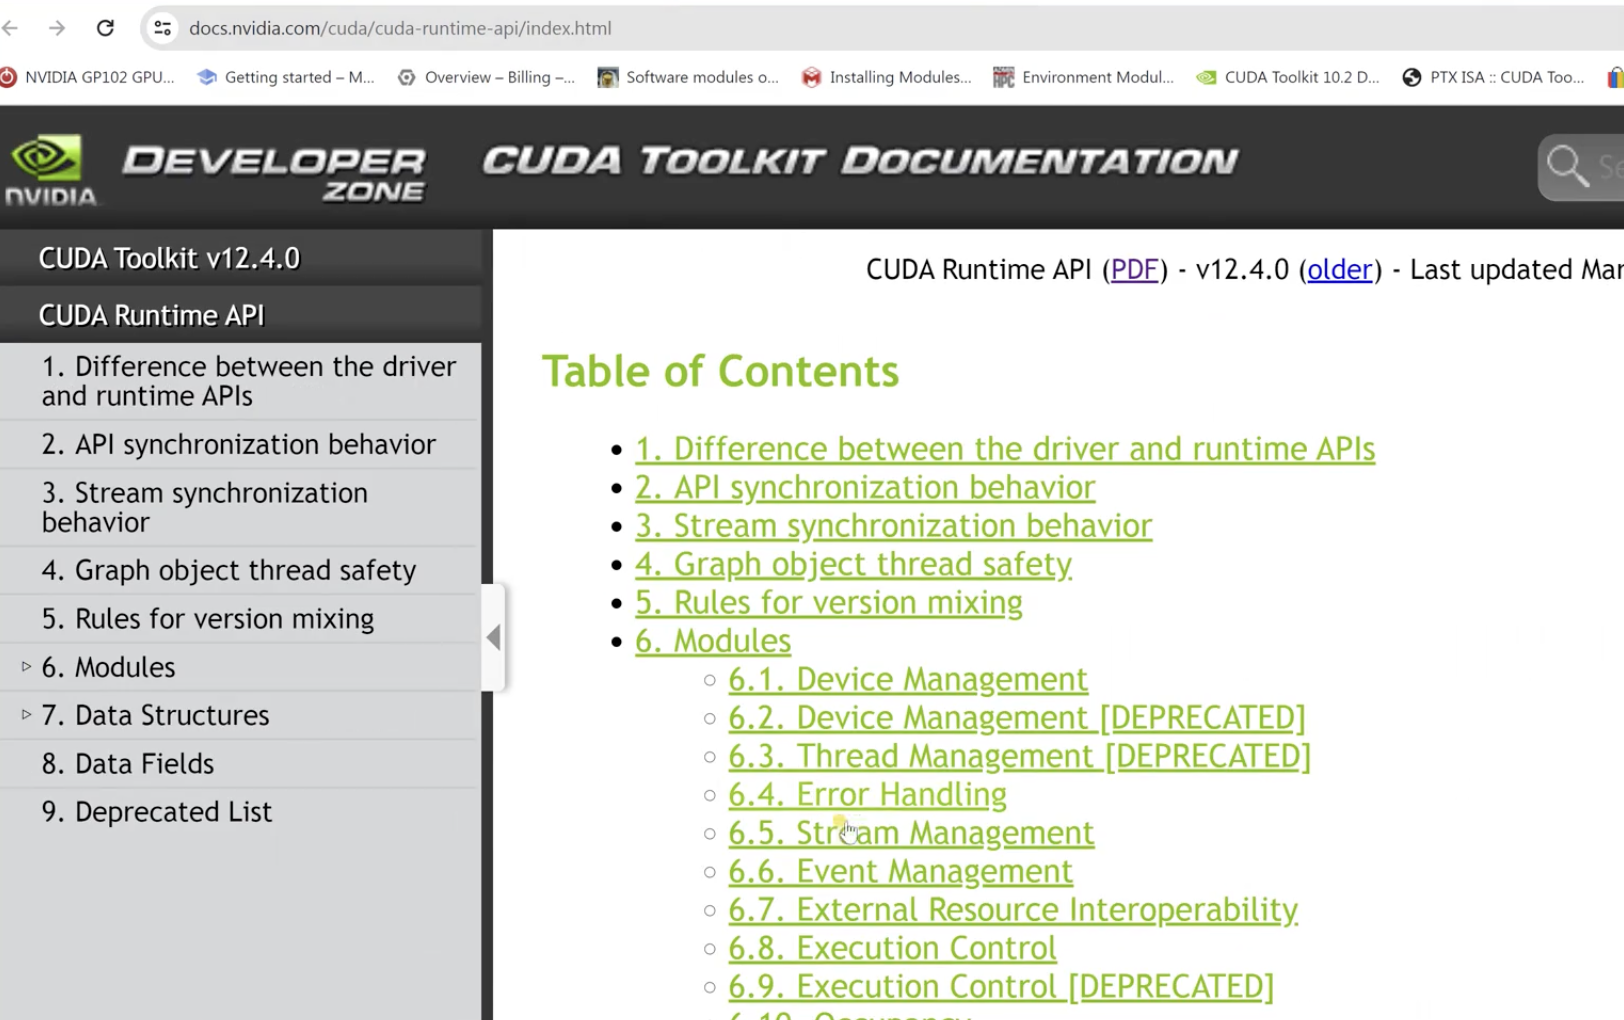
\includegraphics[width=0.75\linewidth]{resources/cuda-081.png}
    \caption{}
    \label{fig:placeholder}
\end{figure}


API函数最常见的例子之一是 \texttt{cudaGetDeviceProperties}函数。该函数旨在查询支持CUDA的GPU（或一般来说NVIDIA 
GPU）的属性和能力。这个函数为开发者提供了重要的信息，例如GPU名称、总全局内存、每个块的最大线程数、
计算能力以及其他指标。这些丰富的信息和指标使开发者能够优化他们的CUDA应用程序。
现在让我们将这个函数应用到我们的GPU上来查询它的属性。

\subsection{项目创建与代码实现}

为了开始我们今天的项目，我们需要进入创建CUDA文件的CUDA课程文件夹，然后从这里创建一个新文件。如我们所见，我选择
了 \texttt{section\_4\_01\_runtime\_api}，但在这里我要删除 \texttt{.txt} 并写上 \texttt{.cu}，
因为我们需要一个 \texttt{.cu}文件，而不是文本文件。然后你需要做的就是来到这里并打开这个文件，
使用任何编辑器（例如Visual StudioCode），然后点击 \texttt{Ctrl+S} 来保存我们的文件。

我要打开它，复制代码并粘贴到这个文件中。这里我想提醒你，这段代码的主要目的是查询GPU的一些属性，我们不需要进行任何计算
。这就是为什么我们在主函数之前没有任何GPU内核，就像我们在所有先前项目中习惯做的那样。

\subsection{代码解析}

\begin{lstlisting}
#include <stdio.h>

int main() {
    int nDevices;

    // 获取系统中可用GPU设备的数量
    cudaGetDeviceCount(&nDevices);

    // 遍历所有设备
    for (int i = 0; i < nDevices; i++) {
        cudaDeviceProp prop;
        
        // 获取设备ID为i的属性
        cudaGetDeviceProperties(&prop, i);

        printf("Device Number: %d\n", i);
        printf("  Device name: %s\n", prop.name);
        printf("  Memory Clock Rate (KHz): %d\n", prop.memoryClockRate);
        printf("  Memory Bus Width (bits): %d\n", prop.memoryBusWidth);
        
        // 峰值内存带宽计算示例（GB/s）
        // 注意：此处读取的是理论峰值而非实际运行值
        double peakBandwidth = 2.0 * prop.memoryClockRate * 
                              (prop.memoryBusWidth / 8) / 1.0e6;
        printf("  Peak Memory Bandwidth (GB/s): %f\n", peakBandwidth);
        
        printf("  Total Global Memory (Bytes): %zu\n", prop.totalGlobalMem);
        printf("  Compute Capability: %d.%d\n", prop.major, prop.minor);
        printf("  SM Count: %d\n", prop.multiProcessorCount);
        
        // 网格与块的限制
        printf("  Max threads per block: %d\n", prop.maxThreadsPerBlock);
        printf("  Max block dims: (%d, %d, %d)\n", 
               prop.maxThreadsDim[0], 
               prop.maxThreadsDim[1], 
               prop.maxThreadsDim[2]);
        printf("  Max grid dims: (%d, %d, %d)\n", 
               prop.maxGridSize[0], 
               prop.maxGridSize[1], 
               prop.maxGridSize[2]);
    }

    return 0;
}
\end{lstlisting}

\begin{figure}
    \centering
    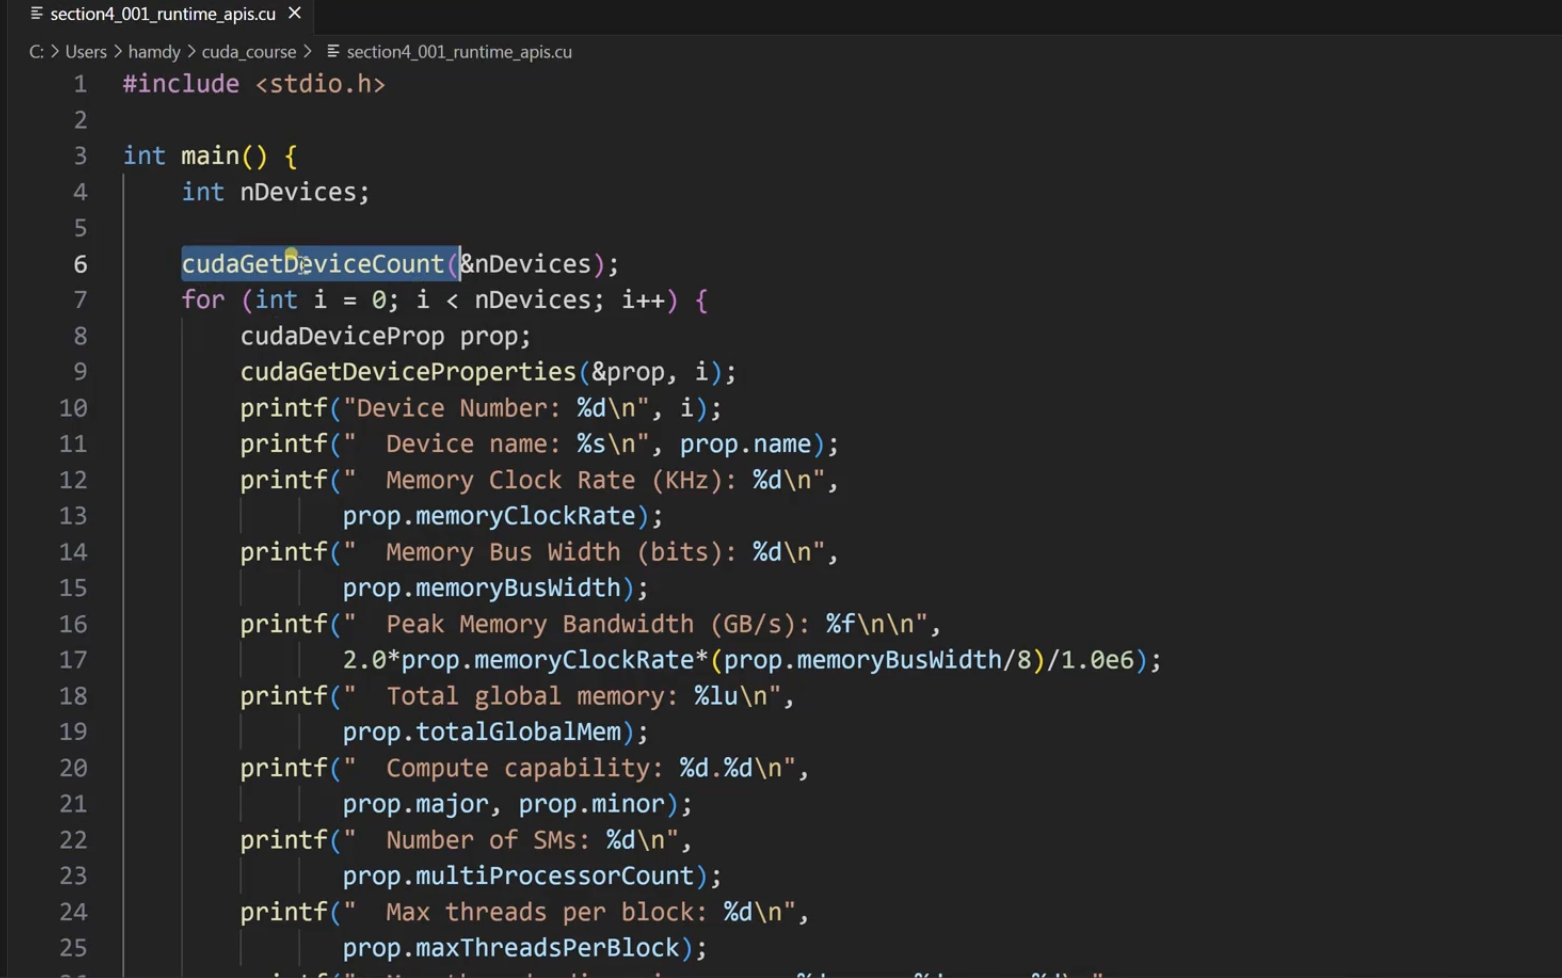
\includegraphics[width=0.75\linewidth]{resources/cuda-082.png}
    \caption{}
    \label{fig:placeholder}
\end{figure}

让我们从这里开始：

\begin{enumerate}
    \item 我们包含 \texttt{stdio.h} 库，以便能够使用 \texttt{printf}。
    \item 声明 \texttt{main} 函数，并为整型变量在内存中分配空间。
    \item 在第6行我们开始使用运行时API函数 \texttt{cudaGetDeviceCount}。函数的名称指的是它的任务：获取系统中设备的数量。如果系统中有3个NVIDIA GPU，那么数字3将存储在 \texttt{nDevices} 中。
    \item 使用 \texttt{for} 循环遍历计算机上所有的设备。我们从 \texttt{i=0} 开始，这指的是GPU编号0。
    \item 创建一个类型为 \texttt{cudaDeviceProp} 的结构体 \texttt{prop}。结构体意味着 \texttt{prop} 将包含不同的值，而不仅仅是一个值。
    \item 使用 \texttt{cudaGetDeviceProperties} 函数读取设备 \texttt{i} 的属性，并将结果存储在 \texttt{prop} 结构体中。
    \item 通过点操作符（\texttt{prop.name}, \texttt{prop.memoryClockRate} 等）访问并打印各项指标。
\end{enumerate}

\subsection{编译与运行验证}

使用NVCC编译器编译代码：

\begin{verbatim}
nvcc -o runtime_api section_4_01_runtime_api.cu
\end{verbatim}

运行可执行文件后，输出示例如下（以RTX 3090为例）：
\begin{itemize}
    \item \textbf{设备编号}: 0
    \item \textbf{设备名称}: GeForce RTX 3090
    \item \textbf{内存总线宽度}: 384 bits（与TechPowerUp数据库一致）
    \item \textbf{总全局内存}: 约24 GB（需将字节数除以 $1024^3$ 转换）
    \item \textbf{计算能力}: 8.6
    \item \textbf{SM数量}: 82
    \item \textbf{每块最大线程数}: 1024
    \item \textbf{最大块维度}: X=1024, Y=1024, Z=64
\end{itemize}

\begin{figure}
    \centering
    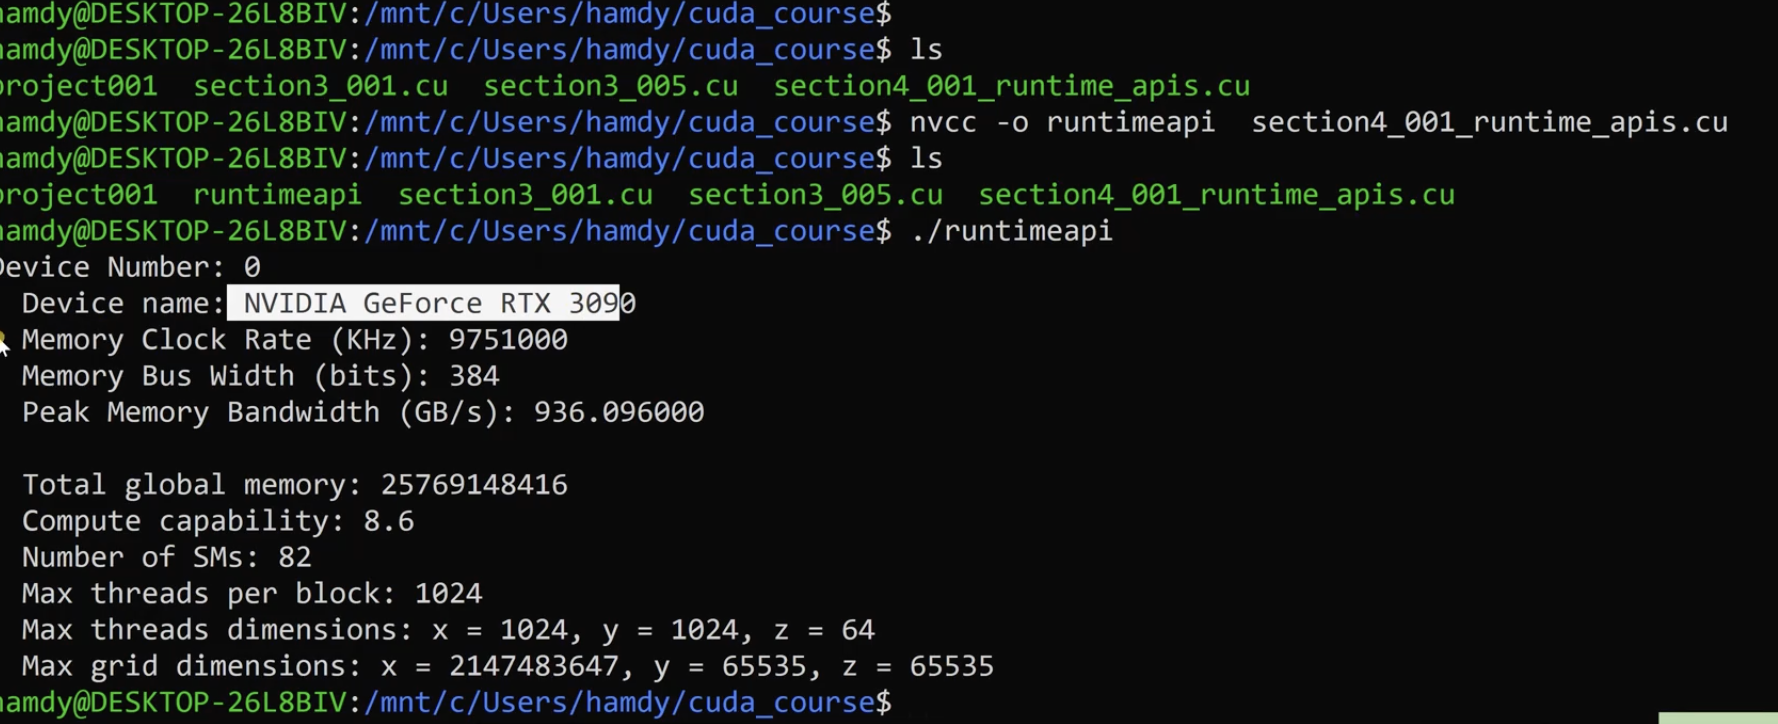
\includegraphics[width=0.75\linewidth]{resources/cuda-083.png}
    \caption{}
    \label{fig:placeholder}
\end{figure}


\textbf{思考题：} 已知每个Warp由32个线程组成，根据每块最大线程数1024，每个块的最大Warp数量是多少
？\[\text{Max Warps per Block} = \frac{1024}{32} = 32\]请注意区分“
块”（软件概念）和“SM”（硬件概念）。块在SM上执行，我们需要这个值来计算另一个性能指标——占用率（Occupancy）。

\subsection{关键要点总结}

\begin{enumerate}
    \item \textbf{参数传递机制}: 运行时API函数的运行方式与标准函数不同。它们不通过典型的返回机制返回结果，而是将输出分配给函数调用中提供的指针参数。例如 \texttt{cudaGetDeviceCount(\&nDevices)} 通过参数存储检测结果。
    
    \item \textbf{错误检查}: 运行时API函数返回它们的执行状态（\texttt{cudaError\_t}），该状态可以被捕获以供后续检查。如果成功则返回 \texttt{cudaSuccess}，否则返回错误代码，可用于分析故障原因。
    
    \item \textbf{效率优势}: 使用运行时API节省了大量时间。替代方案是在白皮书中查阅大量内容才能获取每一个参数值。虽然白皮书中有表格包含许多值，但并非全部，且API能动态反映当前设备的真实状态。
\end{enumerate}

今天就到这里，下个文章见。你需要知道如何使用运行时API，因为在接下来的文章中，我们在检查或分析性能时需要这些值。
